\documentclass[a4paper]{article}

\usepackage[T1]{fontenc}
\usepackage[margin=2.5cm]{geometry}
\usepackage{abstract}
\usepackage{graphicx}

\author{The Unicorn Hunters\\
(Christian Frantzen, Guilherme Barreiro Vieira,\\
Mortimer Sotom and Théo Verhelst )}
\title{Advanced Machine Learning Coursework: Kaggle Competition NYC Taxis}

\begin{document}
\maketitle


\begin{abstract}
This is the abstract
\end{abstract}

\section{Introduction}

\section{Data Analysis}
The first step of a machine learning project is to explore and analyse the data,
in order to better understand the problem. Our dataset is composed of 11
features: a unique identifier for each row, the identifier of the taxi company,
the pickup time, the pickup and drop-off locations, the number of passengers,
and a boolean flag indicated if the trip data has been stored on-board or
directly sent to the data server.

Figures \ref{long} to \ref{pickup_hour} show the distribution of some of these
features. We did not show the pickup month, minute and seconds, as their graphs
are uniformly distributed and therefore not visually informative. Outliers have
been removed in order to properly display the pickup and drop-off location
distribution, as well as the trip duration. These outliers will be discussed in
the next section. We can see in figure \ref{long} and \ref{lat} that the
location seems to be roughly normally distributed, and the logarithm of the trip
duration also appears to be normally distributed in figure
\ref{log_trip_duration}. The smaller bumps outside of the main bell in the
location curves correspond to trips to the city airport.

\begin{figure}
    \centering
   \begin{minipage}{.45\textwidth}
        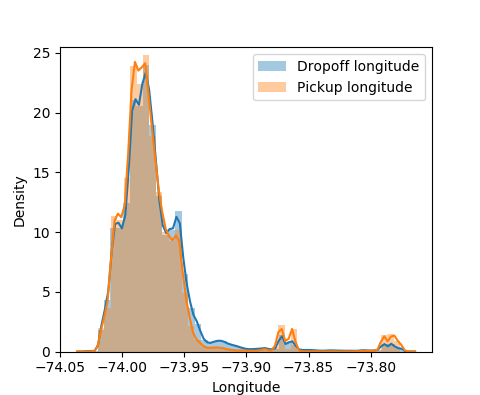
\includegraphics[width=\linewidth]{longitude}
        \caption{Distribtion of the longitude.}
        \label{long}
    \end{minipage}
    \hspace{0.05\textwidth}
    \begin{minipage}{.45\textwidth}
        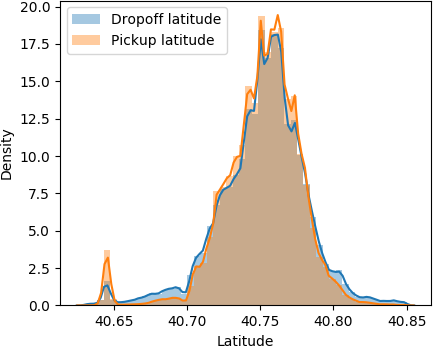
\includegraphics[width=\linewidth]{latitude}
        \caption{Distribution of the latitude.}
        \label{lat}
    \end{minipage}
\end{figure}

\begin{figure}
    \centering
    \begin{minipage}{.45\textwidth}
        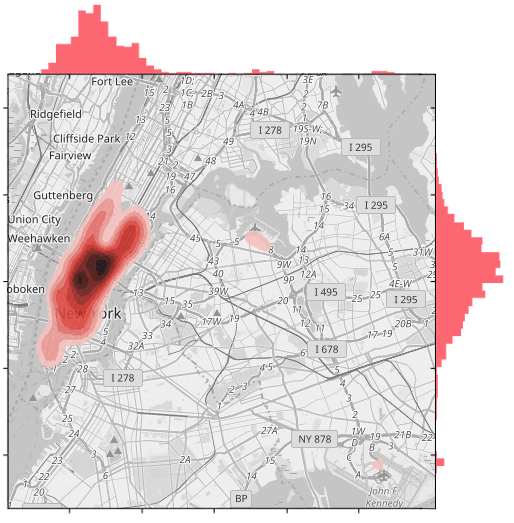
\includegraphics[width=\linewidth]{map_kde}
        \caption{Heatmap of the trip locations on a map (credits: OpenStreeMap).}
        \label{heatmap}
    \end{minipage}
    \hspace{0.05\textwidth}
   \begin{minipage}{.45\textwidth}
       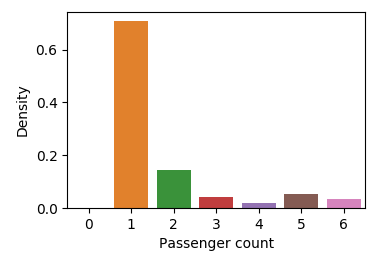
\includegraphics[width=\linewidth]{passenger_count}
       \caption{Distribution of the number of passengers.}
       \label{passenger_count}
    \end{minipage}
\end{figure}

\begin{figure}[h]
    \centering
    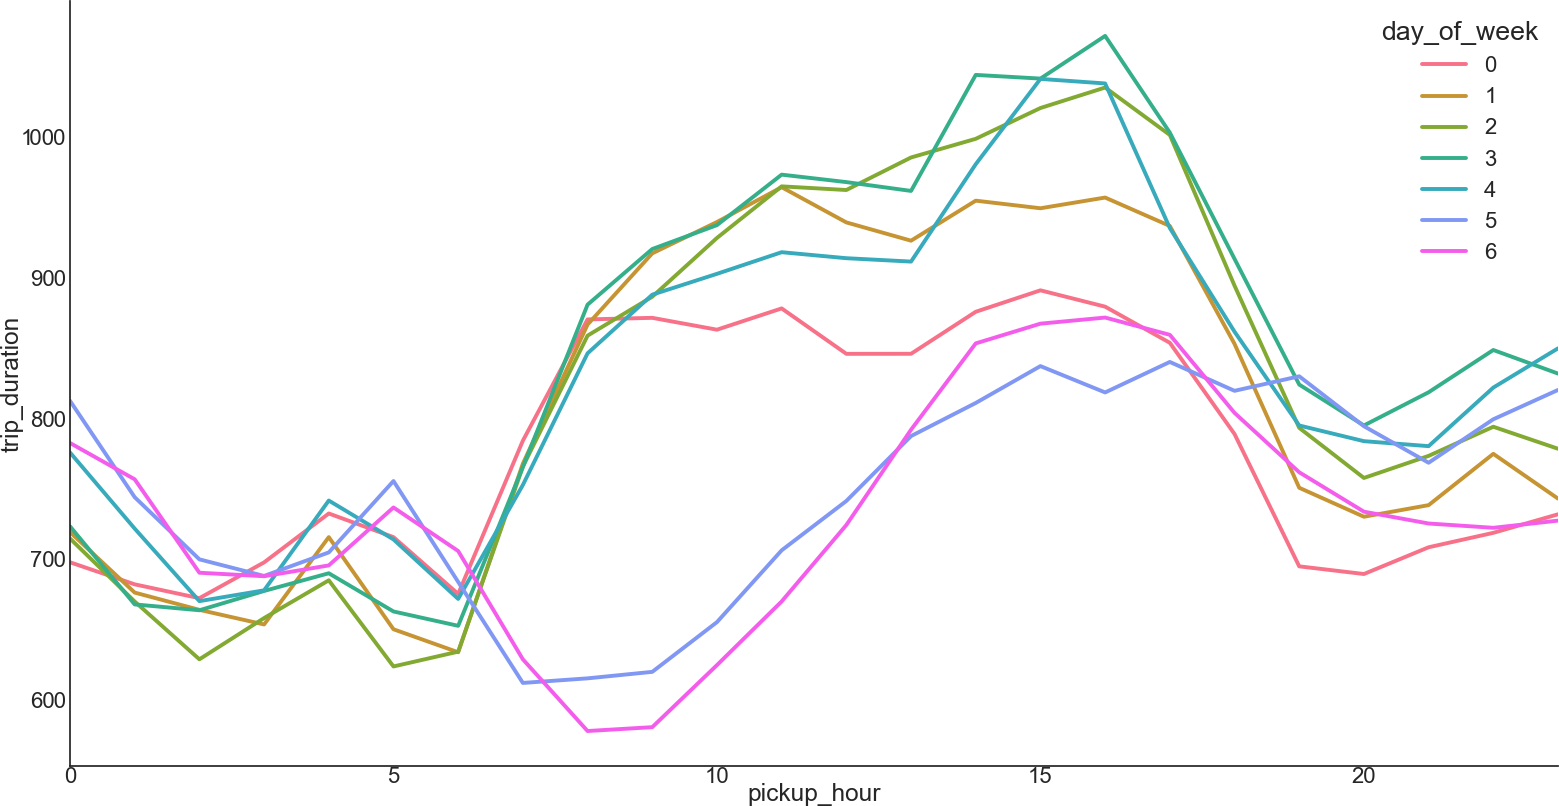
\includegraphics[width=\linewidth]{pickup_hour_vs_trip_duration}
    \caption{Distribution of the pickup time, for different days of the week.}
    \label{pickup_hour}
\end{figure}

\begin{figure}
    \centering
    \begin{minipage}{.45\textwidth}
        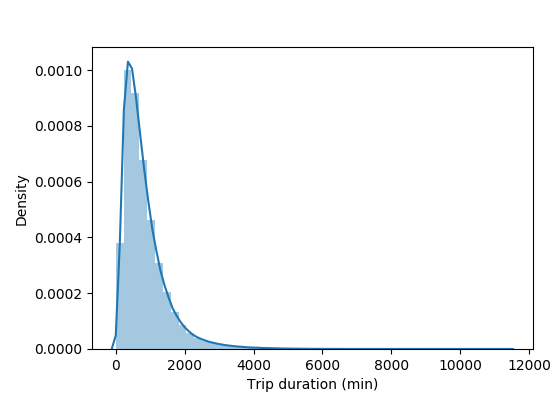
\includegraphics[width=\linewidth]{trip_duration}
        \caption{Distribution of the trip duration, in seconds.}
        \label{trip_duration}
    \end{minipage}
    \hspace{0.05\textwidth}
   \begin{minipage}{.45\textwidth}
       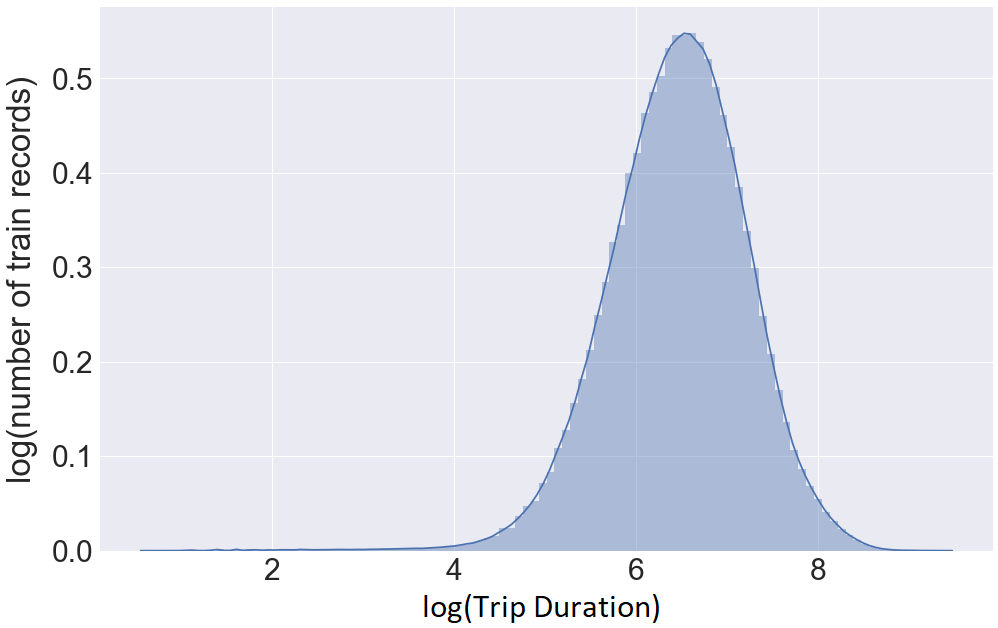
\includegraphics[width=\linewidth]{log_trip_duration}
       \caption{Distribution of the logarithm of the trip duration, in seconds.}
       \label{log_trip_duration}
    \end{minipage}
\end{figure}

 It is also important to make sure that the training and test sets are
independently and identically distributed. For this, we compared the above
distributions with those from the test set. If the distribution from the
training and testing set significantly overlap, then we can consider that the
I.I.D. assumption is verified. As shown for example in figure
\ref{test_vs_train_long} and \ref{test_vs_train_lat}, it is indeed the case.

\begin{figure}
    \centering
    \begin{minipage}{.45\textwidth}
        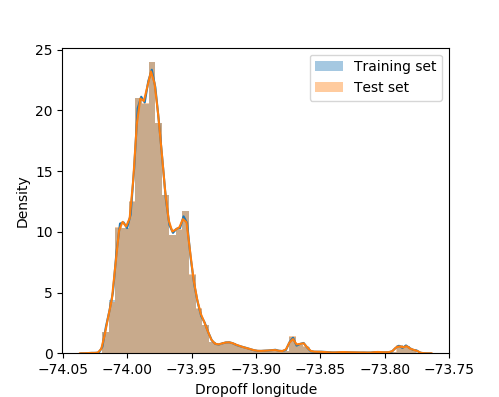
\includegraphics[width=\linewidth]{test_vs_train_long}
        \caption{Drop-off longitude in the training and test set.}
        \label{test_vs_train_long}
    \end{minipage}
    \hspace{0.05\textwidth}
   \begin{minipage}{.45\textwidth}
       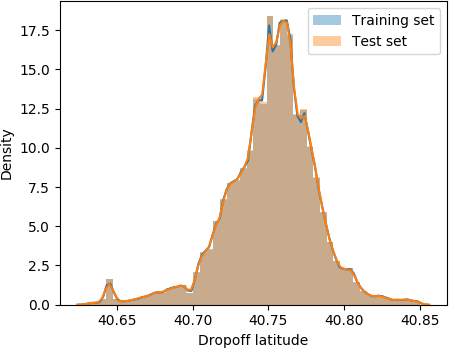
\includegraphics[width=\linewidth]{test_vs_train_lat}
       \caption{Drop-off latitude in the training and test set.}
       \label{test_vs_train_lat}
    \end{minipage}
\end{figure}

\section{Preprocessing}

\section{Feature Selection}
In order to ensure that the model was not being fed useless features, a feature
selection elimination procedure was undertaken. The results are shown in the
above figure - the lower the ranking the better the feature is - by using the
scikit-learn package recursive feature elimination. This function attempted to
find a ranking of the features by doing a prediction while removing one feature
at the time. As expected the most important features such as drop-off and pickup
locations as well as different measures of distance were ranked as very
important. In contrast,  features that didn’t contain much information such as
\texttt{pickup\_year}, \texttt{store\_and\_fwd\_flag}, \texttt{vendor\_id} and
\texttt{pickup\_month}, were ranked as very low importance and hence were
removed from the model. Interestingly enough, the precipitation feature
providing an idea of the weather conditions, didn’t rank very low leading to
believe that it didn’t have a significant effect in the duration of the trips
within New York and specifically Manhattan which is where most of the journeys
were recorded.

\section{Methods for Model Selection}

\section{Results}

\section{Conclusion}

\newpage
\footnotesize
\bibliographystyle{ieeetr}
\bibliography{report}

\appendix
\newpage
\section{Additional Figures}

\end{document}
